\chapter*{Vedlegg A: Spørreundersøkelse}
\label{undersokelse}
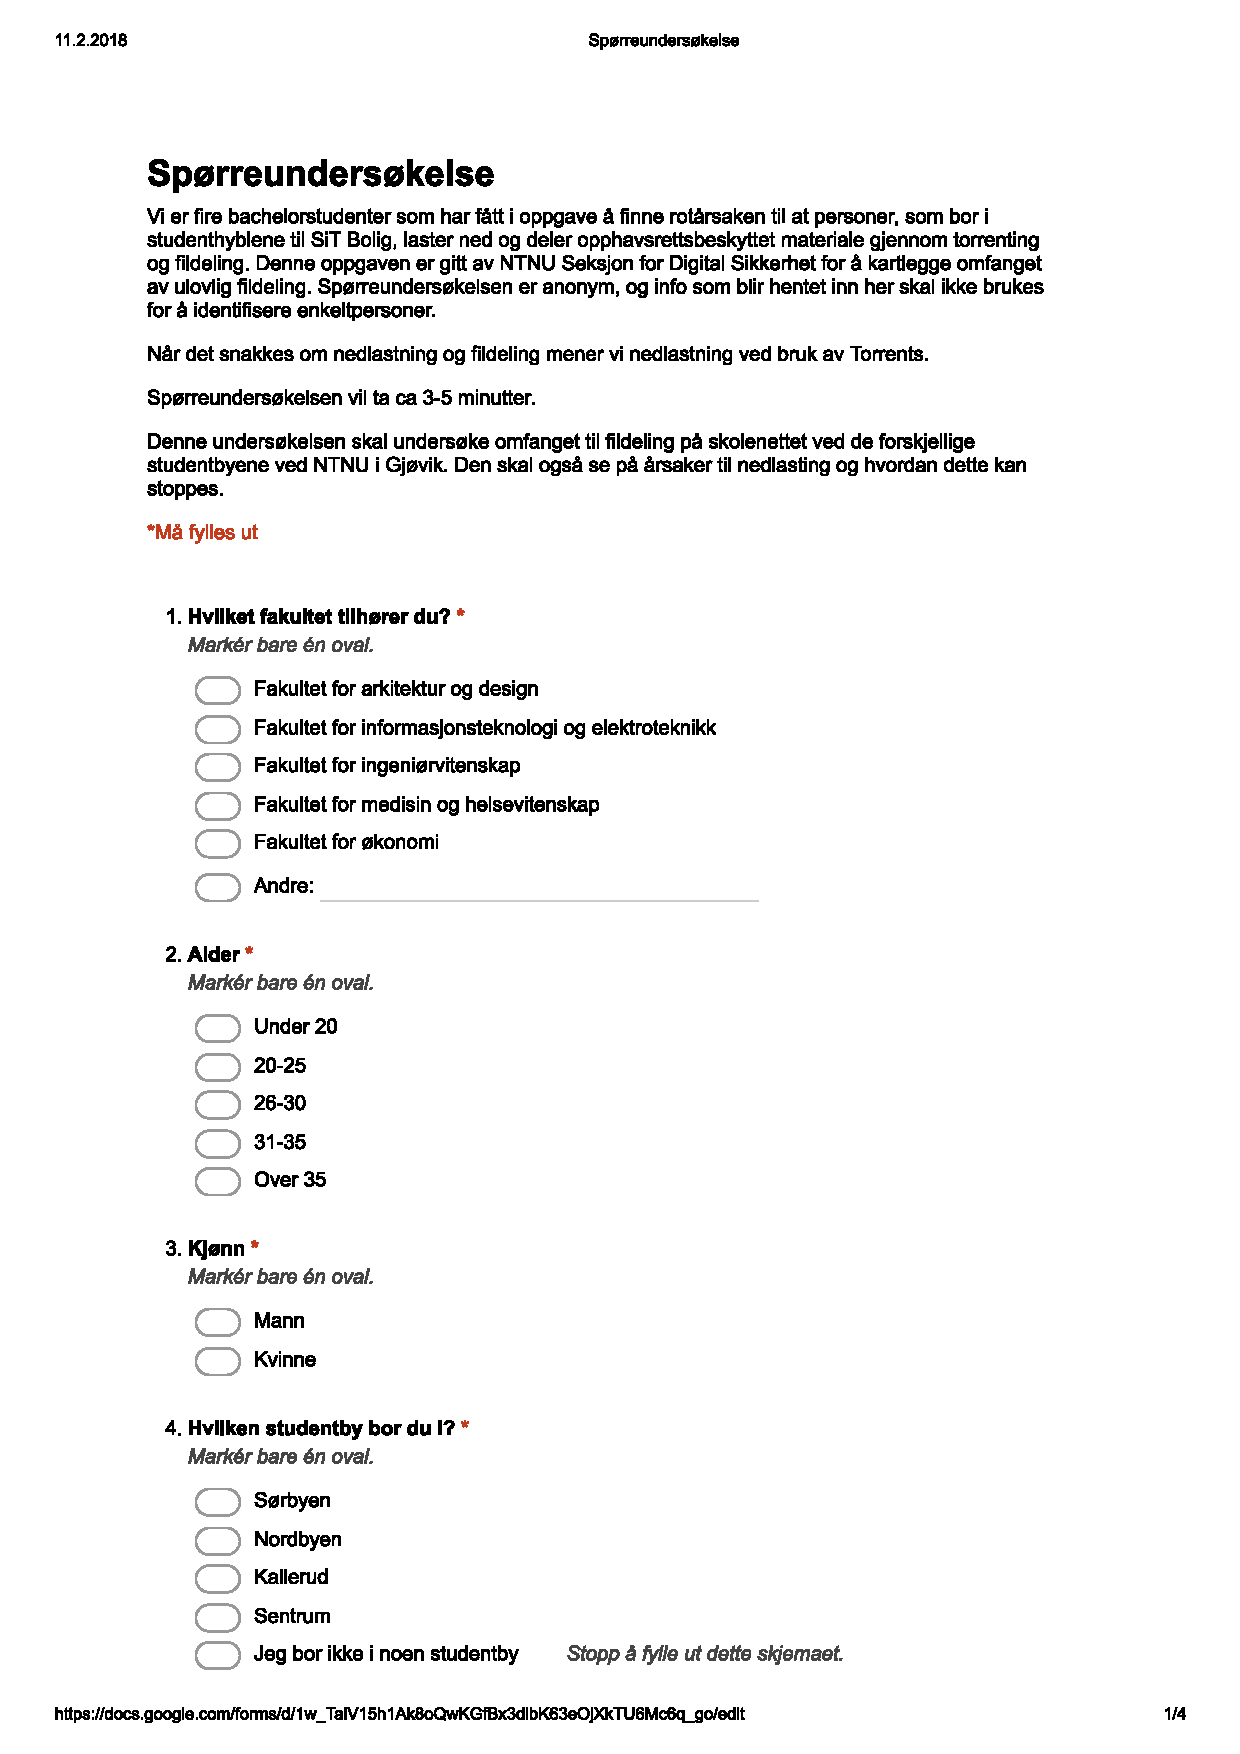
\includepdf[pages={1-4}]{bilder/case1_sporreundersokelse}

\chapter*{Vedlegg B: Plakat}
\label{plakat}
\begin{figure}[H]
    \centering
    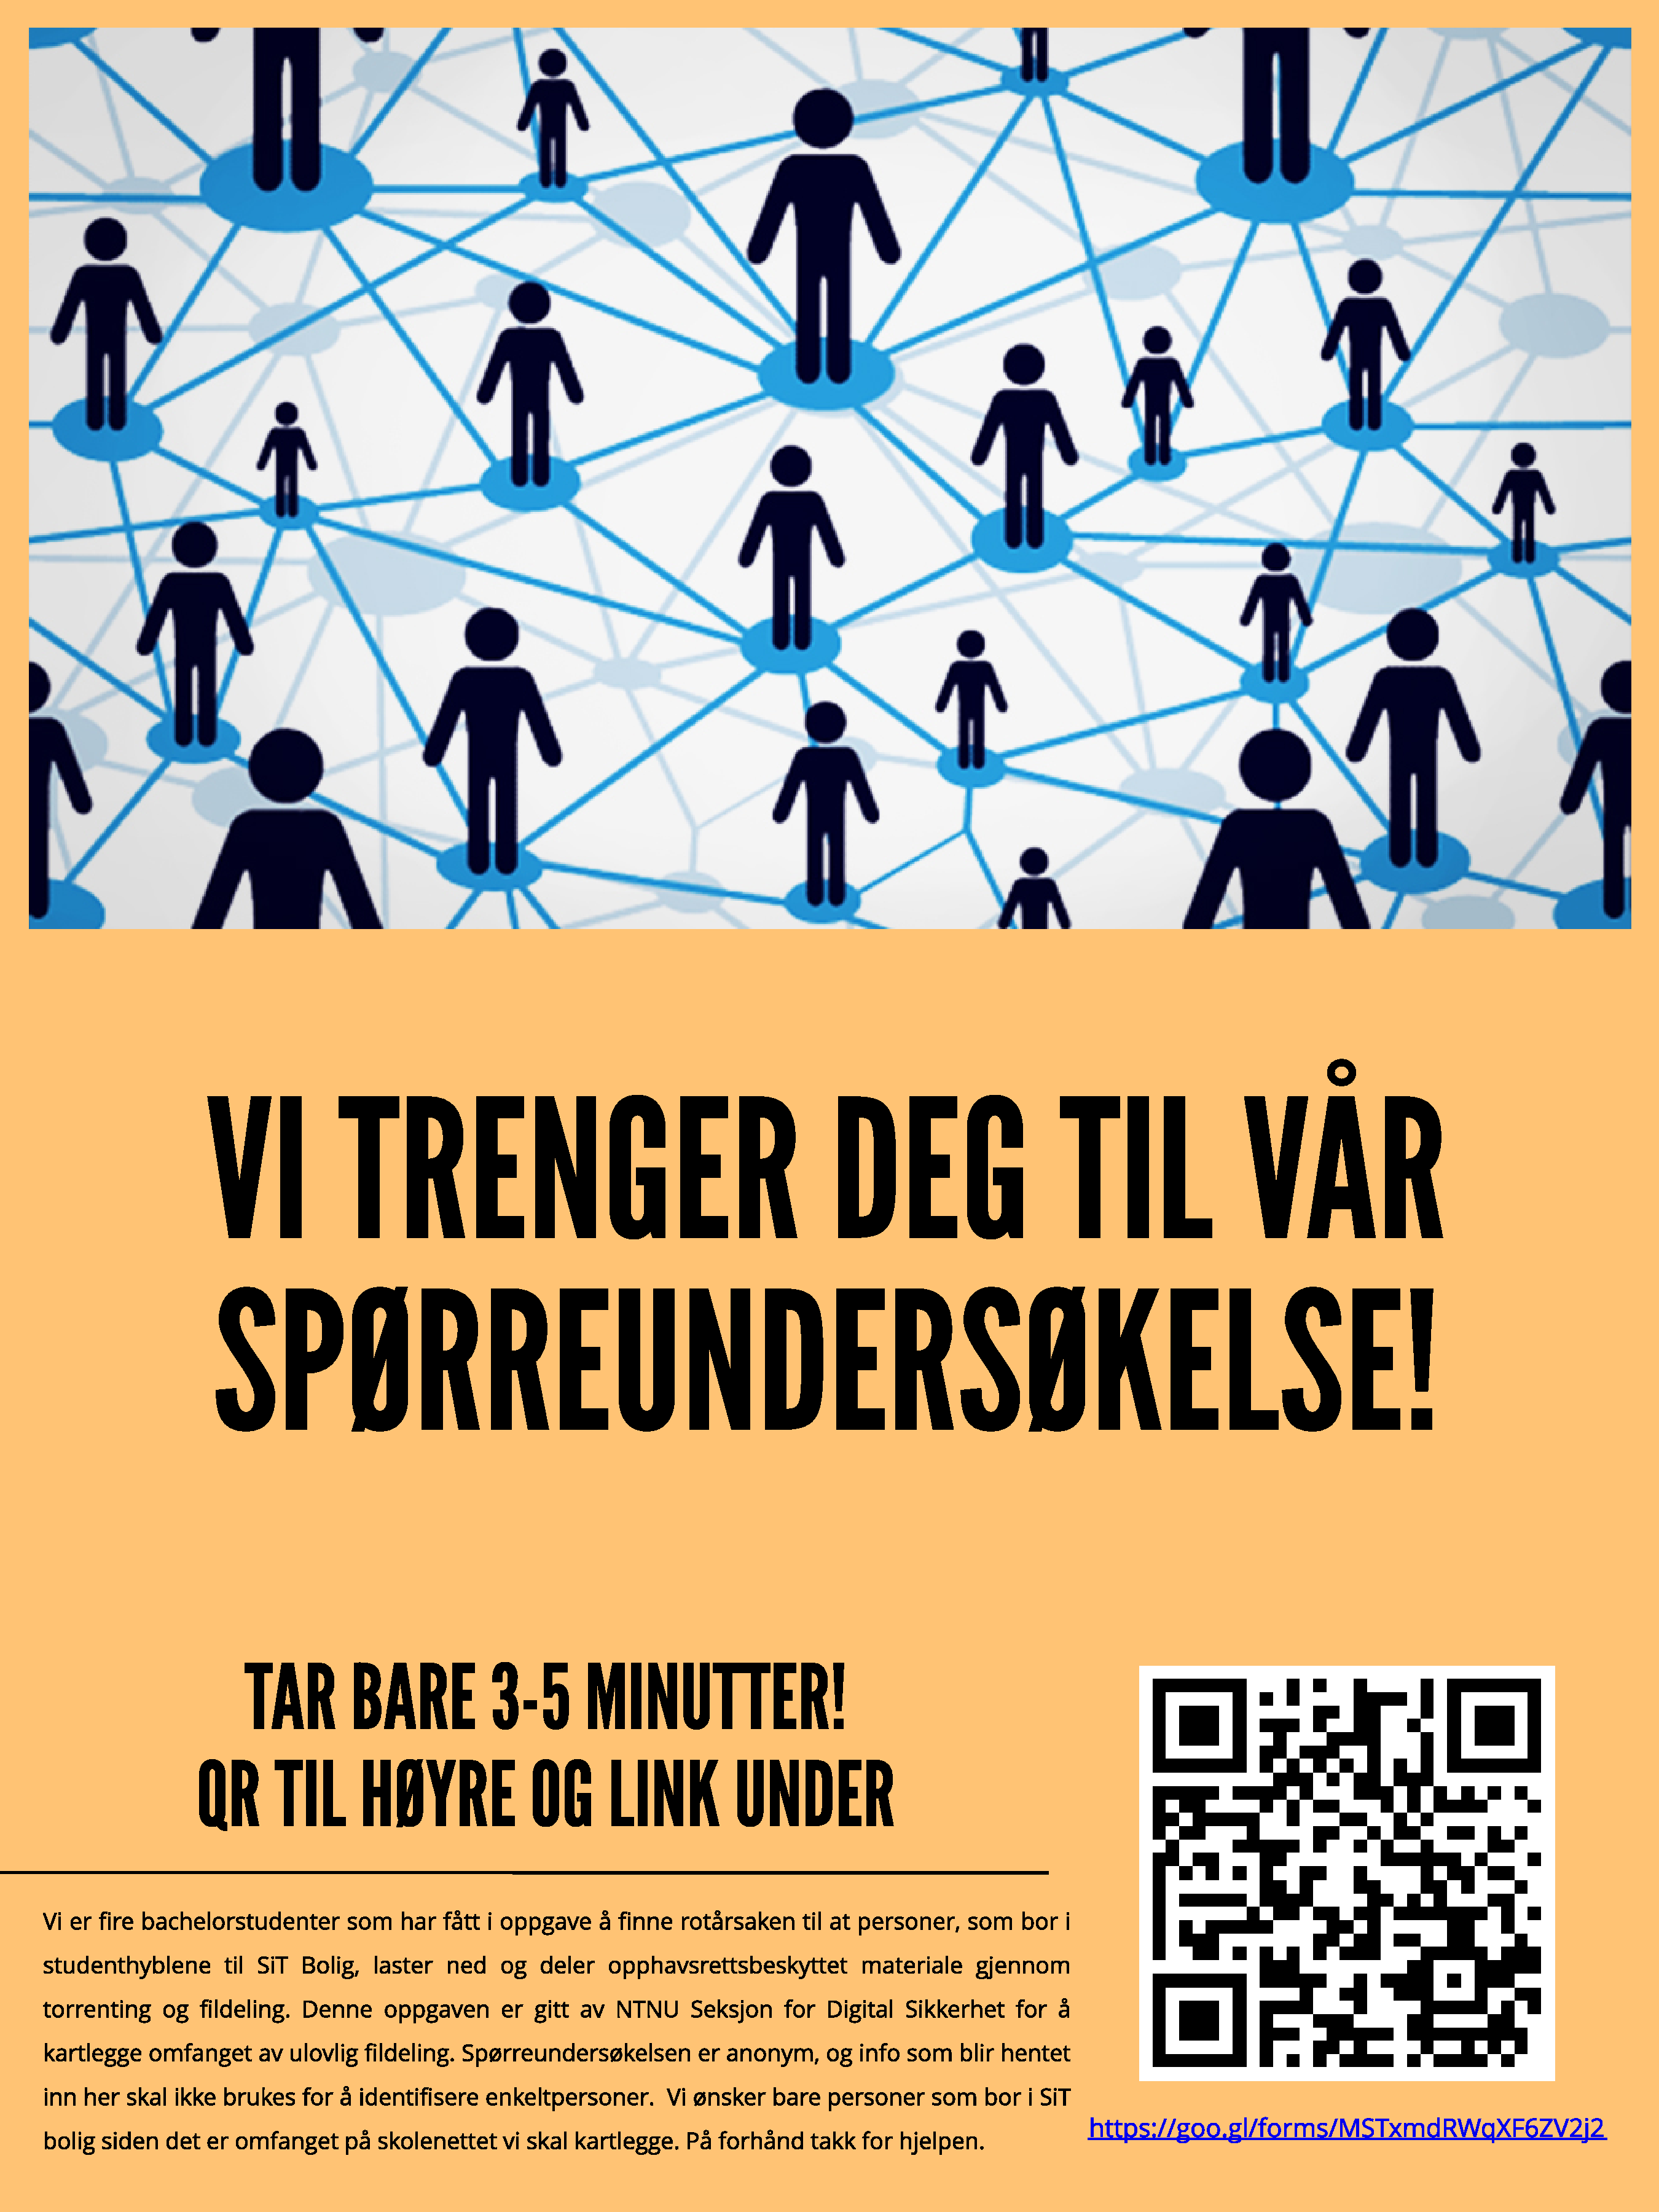
\includegraphics[scale=0.25]{case_1/bilder/plakat.pdf}
    \caption[Plakat]{Plakat som ble brukt i forbindelse med promotering av spørreundersøkelsen}
    \label{fig:plakat}
\end{figure}

\chapter*{Vedlegg C: Frekvenstabeller}
\label{frekvens}

% Table generated by Excel2LaTeX from sheet 'Ark1'
\begin{table}[htbp]
  \centering
    \begin{tabular}{|l|r|r|r|l|}
    \hline
    \multicolumn{5}{|p{30em}|}{\textcolor[rgb]{ .6,  .2,  0}{\textbf{\begin{center}Kjønn\end{center}}}} \\
    \hline
    \textcolor[rgb]{ .2,  .2,  .6}{} & \multicolumn{1}{p{5.355em}|}{\textcolor[rgb]{ .2,  .2,  .6}{Frequency}} & \multicolumn{1}{p{5.355em}|}{\textcolor[rgb]{ .2,  .2,  .6}{Percent}} & \multicolumn{1}{p{5.355em}|}{\textcolor[rgb]{ .2,  .2,  .6}{Valid Percent}} & \multicolumn{1}{p{5.355em}|}{\textcolor[rgb]{ .2,  .2,  .6}{Cumulative Percent}} \\
    \hline
    \textcolor[rgb]{ .2,  .2,  .6}{Kvinne} & \textcolor[rgb]{ .6,  .2,  0}{27} & \textcolor[rgb]{ .6,  .2,  0}{27.8} & \textcolor[rgb]{ .6,  .2,  0}{27.8} & \multicolumn{1}{r|}{\textcolor[rgb]{ .6,  .2,  0}{27.8}} \\
    \hline
    \textcolor[rgb]{ .2,  .2,  .6}{Mann}  & \textcolor[rgb]{ .6,  .2,  0}{70} & \textcolor[rgb]{ .6,  .2,  0}{72.2} & \textcolor[rgb]{ .6,  .2,  0}{72.2} & \multicolumn{1}{r|}{\textcolor[rgb]{ .6,  .2,  0}{100.0}} \\
    \hline
    \textcolor[rgb]{ .2,  .2,  .6}{Total} & \textcolor[rgb]{ .6,  .2,  0}{97} & \textcolor[rgb]{ .6,  .2,  0}{100.0} & \textcolor[rgb]{ .6,  .2,  0}{100.0} & \textcolor[rgb]{ .6,  .2,  0}{} \\
    \hline
    \end{tabular}%
  \caption{Frekvenstabell av kjønn}
  \label{tab:kjonn}%
\end{table}%

\begin{table}[htbp]
  \centering
    \begin{tabular}{|l|r|r|r|l|}
    \hline
    \multicolumn{5}{|p{30em}|}{\textcolor[rgb]{ .6,  .2,  0}{\textbf{\begin{center}Alder\end{center}}}} \\
    \hline
    \textcolor[rgb]{ .2,  .2,  .6}{} & \multicolumn{1}{p{5.355em}|}{\textcolor[rgb]{ .2,  .2,  .6}{Frequency}} & \multicolumn{1}{p{5.355em}|}{\textcolor[rgb]{ .2,  .2,  .6}{Percent}} & \multicolumn{1}{p{5.355em}|}{\textcolor[rgb]{ .2,  .2,  .6}{Valid Percent}} & \multicolumn{1}{p{5.355em}|}{\textcolor[rgb]{ .2,  .2,  .6}{Cumulative Percent}} \\
    \hline
    \textcolor[rgb]{ .2,  .2,  .6}{Under 20} & \textcolor[rgb]{ .6,  .2,  0}{9} & \textcolor[rgb]{ .6,  .2,  0}{9.3} & \textcolor[rgb]{ .6,  .2,  0}{9.3} & \multicolumn{1}{r|}{\textcolor[rgb]{ .6,  .2,  0}{9.3}} \\
    \hline
    \textcolor[rgb]{ .2,  .2,  .6}{20-25}  & \textcolor[rgb]{ .6,  .2,  0}{72} & \textcolor[rgb]{ .6,  .2,  0}{74.2} & \textcolor[rgb]{ .6,  .2,  0}{74.2} & \multicolumn{1}{r|}{\textcolor[rgb]{ .6,  .2,  0}{83.5}} \\
    \hline
    \textcolor[rgb]{ .2,  .2,  .6}{26-30} & \textcolor[rgb]{ .6,  .2,  0}{11} & \textcolor[rgb]{ .6,  .2,  0}{11.3} & \textcolor[rgb]{ .6,  .2,  0}{11.3} & \multicolumn{1}{r|}{\textcolor[rgb]{ .6,  .2,  0}{94.9}} \\
    \hline
    \textcolor[rgb]{ .2,  .2,  .6}{31-35} & \textcolor[rgb]{ .6,  .2,  0}{4} & \textcolor[rgb]{ .6,  .2,  0}{4.1} & \textcolor[rgb]{ .6,  .2,  0}{4.1} & \multicolumn{1}{r|}{\textcolor[rgb]{ .6,  .2,  0}{99.0}} \\
    \hline
    \textcolor[rgb]{ .2,  .2,  .6}{Over 35} & \textcolor[rgb]{ .6,  .2,  0}{1} & \textcolor[rgb]{ .6,  .2,  0}{1.0} & \textcolor[rgb]{ .6,  .2,  0}{1.0} & \multicolumn{1}{r|}{\textcolor[rgb]{ .6,  .2,  0}{100.0}} \\
    \hline
    \textcolor[rgb]{ .2,  .2,  .6}{Total} & \textcolor[rgb]{ .6,  .2,  0}{97} & \textcolor[rgb]{ .6,  .2,  0}{100.0} & \textcolor[rgb]{ .6,  .2,  0}{100.0} & \multicolumn{1}{r|}{\textcolor[rgb]{ .6,  .2,  0}{}} \\
    \hline
    \end{tabular}%
  \caption{Frekvenstabell av alder}
  \label{tab:alder}%
\end{table}%

\begin{table}[htbp]
  \centering
    \begin{tabular}{|l|r|r|r|l|}
    \hline
    \multicolumn{5}{|p{30em}|}{\textcolor[rgb]{ .6,  .2,  0}{\textbf{\begin{center}Studentby\end{center}}}} \\
    \hline
    \textcolor[rgb]{ .2,  .2,  .6}{} & \multicolumn{1}{p{5.355em}|}{\textcolor[rgb]{ .2,  .2,  .6}{Frequency}} & \multicolumn{1}{p{5.355em}|}{\textcolor[rgb]{ .2,  .2,  .6}{Percent}} & \multicolumn{1}{p{5.355em}|}{\textcolor[rgb]{ .2,  .2,  .6}{Valid Percent}} & \multicolumn{1}{p{5.355em}|}{\textcolor[rgb]{ .2,  .2,  .6}{Cumulative Percent}} \\
    \hline
    \textcolor[rgb]{ .2,  .2,  .6}{Kallerud} & \textcolor[rgb]{ .6,  .2,  0}{49} & \textcolor[rgb]{ .6,  .2,  0}{50.5} & \textcolor[rgb]{ .6,  .2,  0}{50.5} & \multicolumn{1}{r|}{\textcolor[rgb]{ .6,  .2,  0}{50.5}} \\
    \hline
    \textcolor[rgb]{ .2,  .2,  .6}{Nordbyen}  & \textcolor[rgb]{ .6,  .2,  0}{13} & \textcolor[rgb]{ .6,  .2,  0}{13.4} & \textcolor[rgb]{ .6,  .2,  0}{13.4} & \multicolumn{1}{r|}{\textcolor[rgb]{ .6,  .2,  0}{63.9}} \\
    \hline
    \textcolor[rgb]{ .2,  .2,  .6}{Sentrum} & \textcolor[rgb]{ .6,  .2,  0}{11} & \textcolor[rgb]{ .6,  .2,  0}{11.3} & \textcolor[rgb]{ .6,  .2,  0}{11.3} & \multicolumn{1}{r|}{\textcolor[rgb]{ .6,  .2,  0}{75.3}} \\
    \hline
    \textcolor[rgb]{ .2,  .2,  .6}{Sørbyen} & \textcolor[rgb]{ .6,  .2,  0}{24} & \textcolor[rgb]{ .6,  .2,  0}{24.7} & \textcolor[rgb]{ .6,  .2,  0}{24.7} & \multicolumn{1}{r|}{\textcolor[rgb]{ .6,  .2,  0}{100.0}} \\
    \hline
    \textcolor[rgb]{ .2,  .2,  .6}{Total} & \textcolor[rgb]{ .6,  .2,  0}{97} & \textcolor[rgb]{ .6,  .2,  0}{100.0} & \textcolor[rgb]{ .6,  .2,  0}{100.0} & \multicolumn{1}{r|}{\textcolor[rgb]{ .6,  .2,  0}{}} \\
    \hline
    \end{tabular}%
  \caption{Frekvenstabell av studentby}
  \label{tab:studentby}%
\end{table}%

\begin{table}[htbp]
  \centering
    \begin{tabular}{|p{5.355em}|r|r|r|l|}
    \hline
    \multicolumn{5}{|p{30em}|}{\textcolor[rgb]{ .6,  .2,  0}{\textbf{\begin{center}Fakultet\end{center}}}} \\
    \hline
    \multicolumn{1}{|r|}{\textcolor[rgb]{ .2,  .2,  .6}{}} & \multicolumn{1}{p{5.355em}|}{\textcolor[rgb]{ .2,  .2,  .6}{Frequency}} & \multicolumn{1}{p{5.355em}|}{\textcolor[rgb]{ .2,  .2,  .6}{Percent}} & \multicolumn{1}{p{5.355em}|}{\textcolor[rgb]{ .2,  .2,  .6}{Valid Percent}} & \multicolumn{1}{p{5.355em}|}{\textcolor[rgb]{ .2,  .2,  .6}{Cumulative Percent}} \\
    \hline
    \textcolor[rgb]{ .2,  .2,  .6}{Fakultet for arkitektur og design} & \textcolor[rgb]{ .6,  .2,  0}{15} & \textcolor[rgb]{ .6,  .2,  0}{15.5} & \textcolor[rgb]{ .6,  .2,  0}{15.5} & \multicolumn{1}{r|}{\textcolor[rgb]{ .6,  .2,  0}{15.5}} \\
    \hline
    \textcolor[rgb]{ .2,  .2,  .6}{Fakultet for informasjonsteknologi og elektroteknikk} & \textcolor[rgb]{ .6,  .2,  0}{52} & \textcolor[rgb]{ .6,  .2,  0}{53.6} & \textcolor[rgb]{ .6,  .2,  0}{53.6} & \multicolumn{1}{r|}{\textcolor[rgb]{ .6,  .2,  0}{69.1}} \\
    \hline
    \textcolor[rgb]{ .2,  .2,  .6}{Fakultet for ingeniørvitenskap} & \textcolor[rgb]{ .6,  .2,  0}{13} & \textcolor[rgb]{ .6,  .2,  0}{13.4} & \textcolor[rgb]{ .6,  .2,  0}{13.4} & \multicolumn{1}{r|}{\textcolor[rgb]{ .6,  .2,  0}{82.5}} \\
    \hline
    \textcolor[rgb]{ .2,  .2,  .6}{Fakultet for medisin og helsevitenskap} & \textcolor[rgb]{ .6,  .2,  0}{11} & \textcolor[rgb]{ .6,  .2,  0}{11.3} & \textcolor[rgb]{ .6,  .2,  0}{11.3} & \multicolumn{1}{r|}{\textcolor[rgb]{ .6,  .2,  0}{93.8}} \\
    \hline
    \textcolor[rgb]{ .2,  .2,  .6}{Fakultet for økonomi} & \textcolor[rgb]{ .6,  .2,  0}{6} & \textcolor[rgb]{ .6,  .2,  0}{6.2} & \textcolor[rgb]{ .6,  .2,  0}{6.2} & \multicolumn{1}{r|}{\textcolor[rgb]{ .6,  .2,  0}{100.0}} \\   
    \hline
    \textcolor[rgb]{ .2,  .2,  .6}{Total} & \textcolor[rgb]{ .6,  .2,  0}{97} & \textcolor[rgb]{ .6,  .2,  0}{100.0} & \textcolor[rgb]{ .6,  .2,  0}{100.0} & \textcolor[rgb]{ .6,  .2,  0}{} \\
    \hline
    \end{tabular}%
  \caption{Frekvenstabell av fakultet}
  \label{tab:fakultet}%
\end{table}%

\chapter*{Vedlegg D: Diverse Histogrammer}
\label{vedlegg:histogrammer}

\begin{figure}[H]
    \centering
    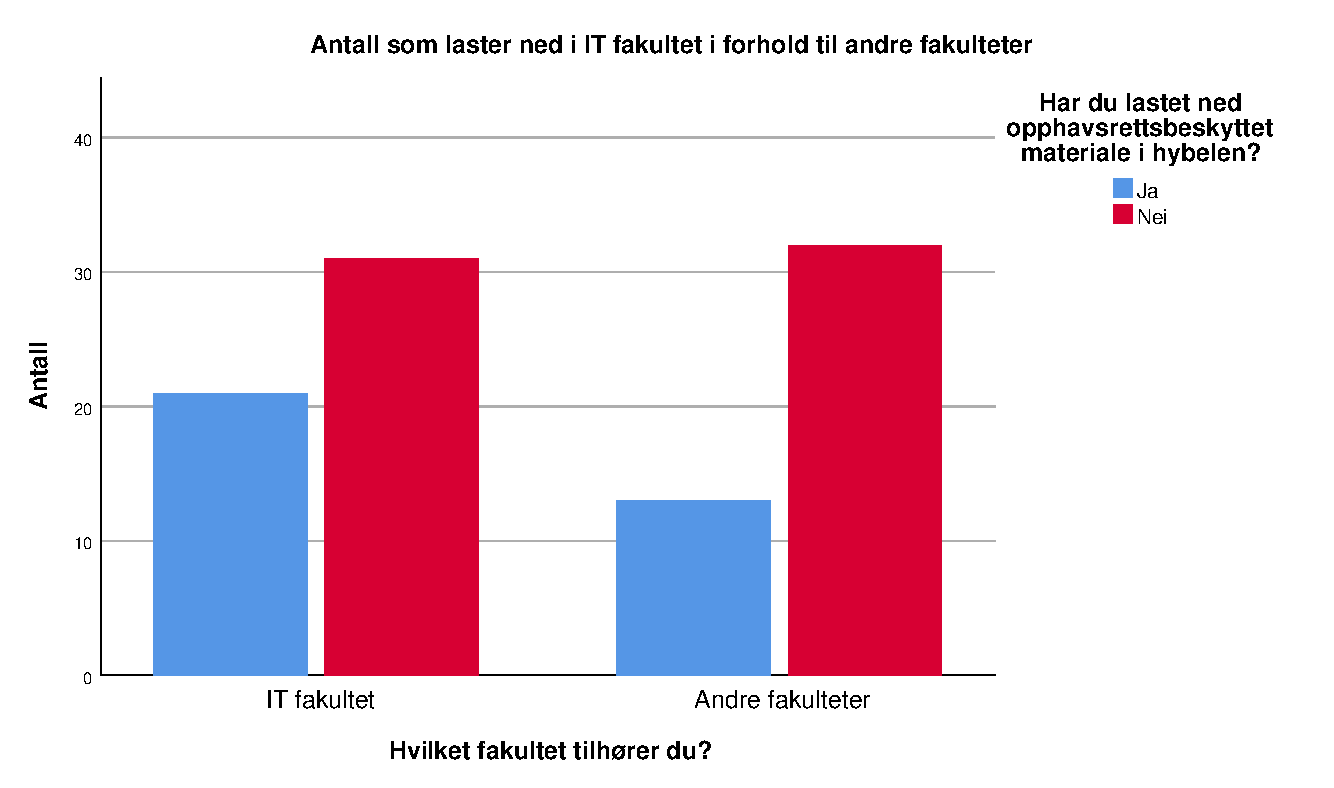
\includegraphics[scale=0.45]{case_1/bilder/IT_lasterned.pdf}
    \caption[IT-lasterned]{Forholdet mellom IT studier og andre når det kommer til nedlasting}
    \label{fig:IT-lasterned}
\end{figure}

\begin{figure}[H]
    \centering
    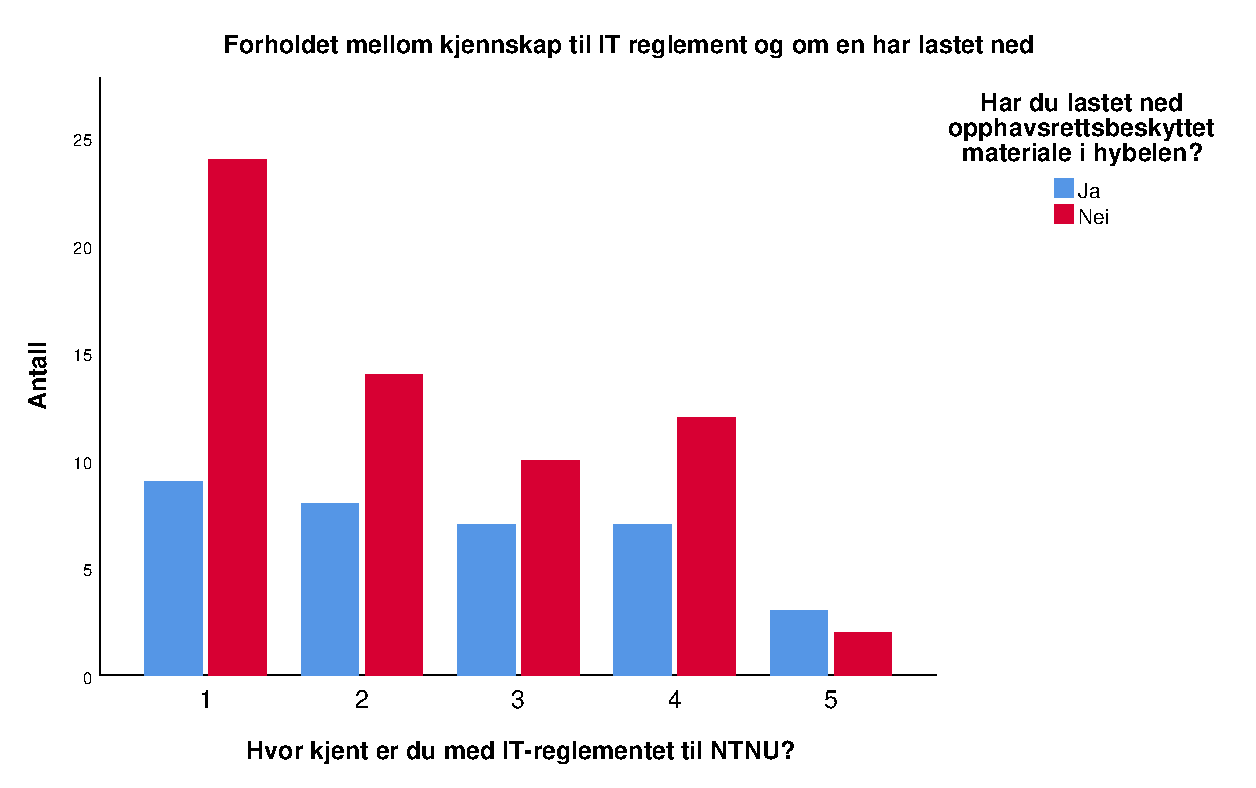
\includegraphics[scale=0.45]{case_1/bilder/reglement_lasterned.pdf}
    \caption[reglement-lasterned]{Forholdet mellom kjennskap til IT reglement og om en laster ned}
    \label{fig:reglement-lasterned}
\end{figure}

\begin{figure}[H]
    \centering
    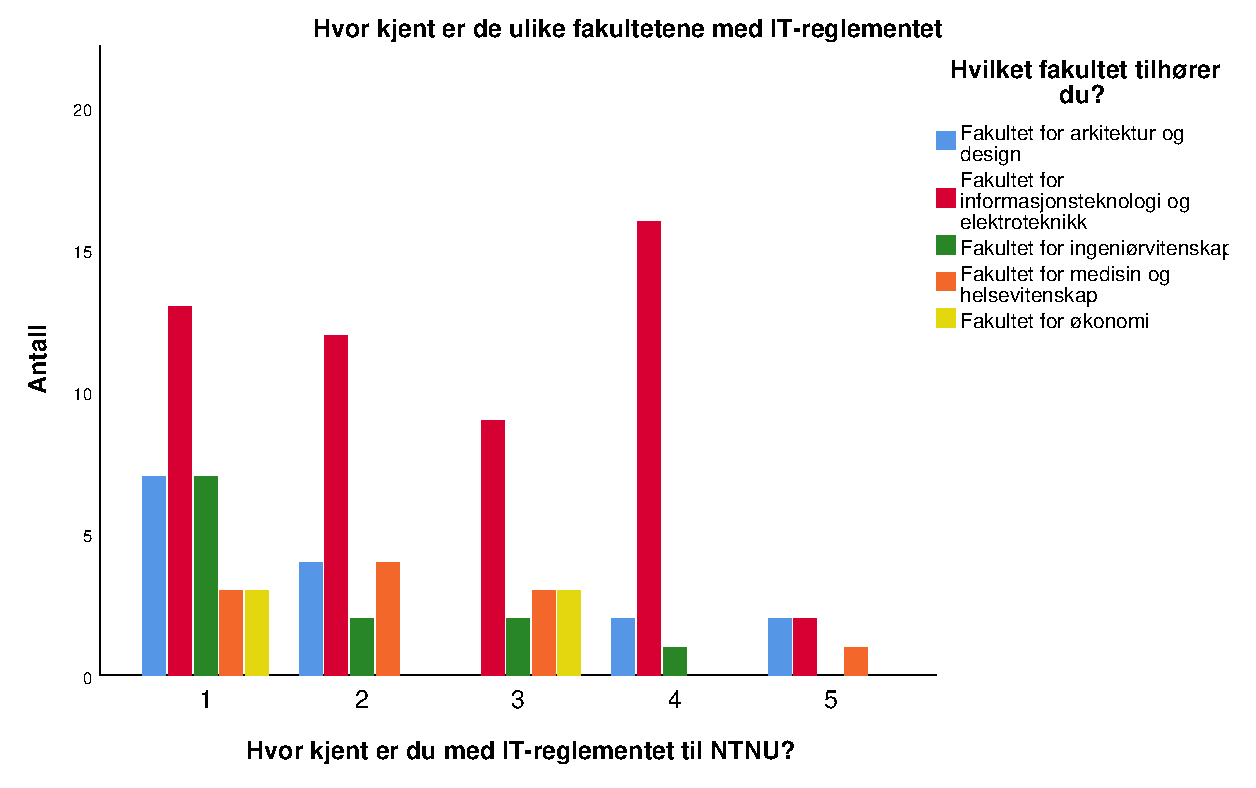
\includegraphics[scale=0.45]{case_1/bilder/reglement_fakultet.pdf}
    \caption[reglement-fakultet]{Hvor godt kjennskap de ulike fakultetene har med IT reglementet}
    \label{fig:reglement-fakultet}
\end{figure}

\begin{figure}[H]
    \centering
    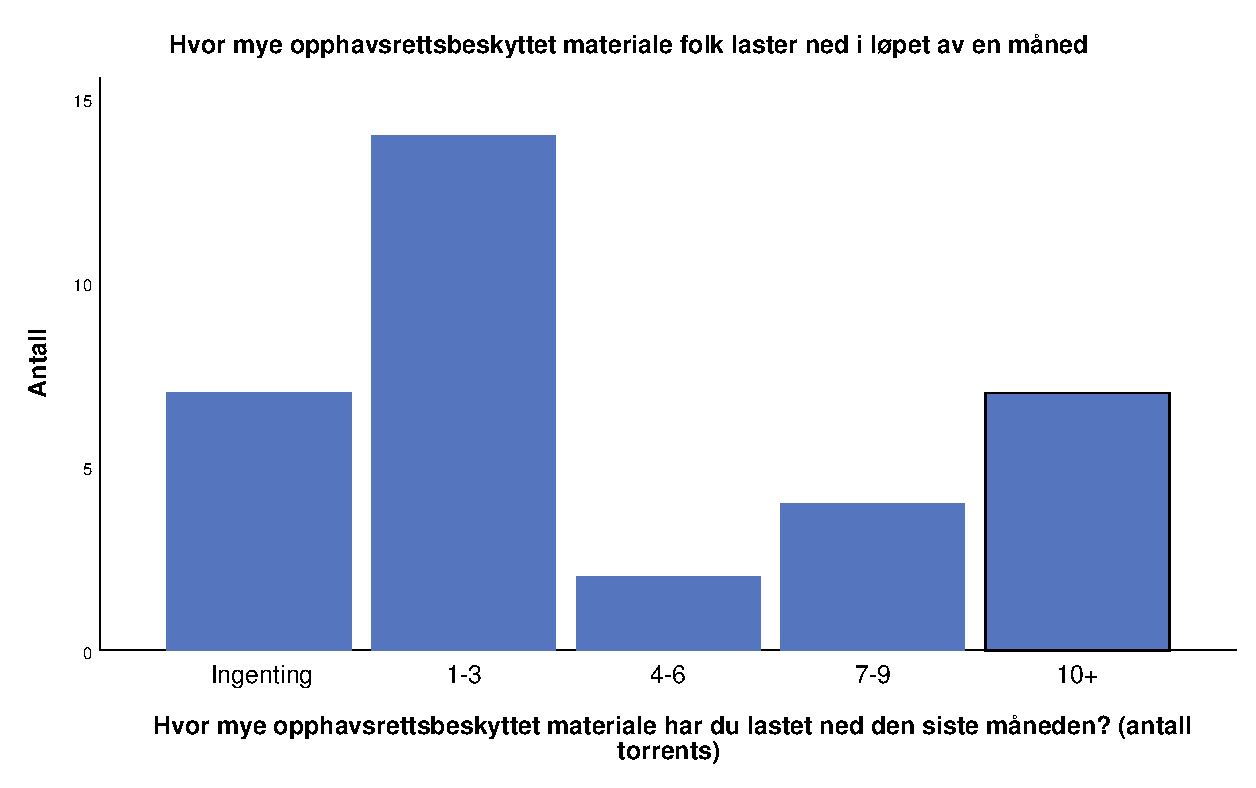
\includegraphics[scale=0.45]{case_1/bilder/antalltorrents.pdf}
    \caption[antalltorrents]{Hvor mange torrents folk laster ned i løpet av en måned}
    \label{fig:antalltorrents}
\end{figure}

\chapter*{Vedlegg E: SPSS analyser}
\label{vedlegg:ANOVA}

%-----------------------------------------------ONEWAY ANOVA - FAKULTET MOT PÅSTAND------------------------
%-----------------------------------------------DESCRIPTIVES-----------------------------------------------
\begin{figure}[H]
    \centering
    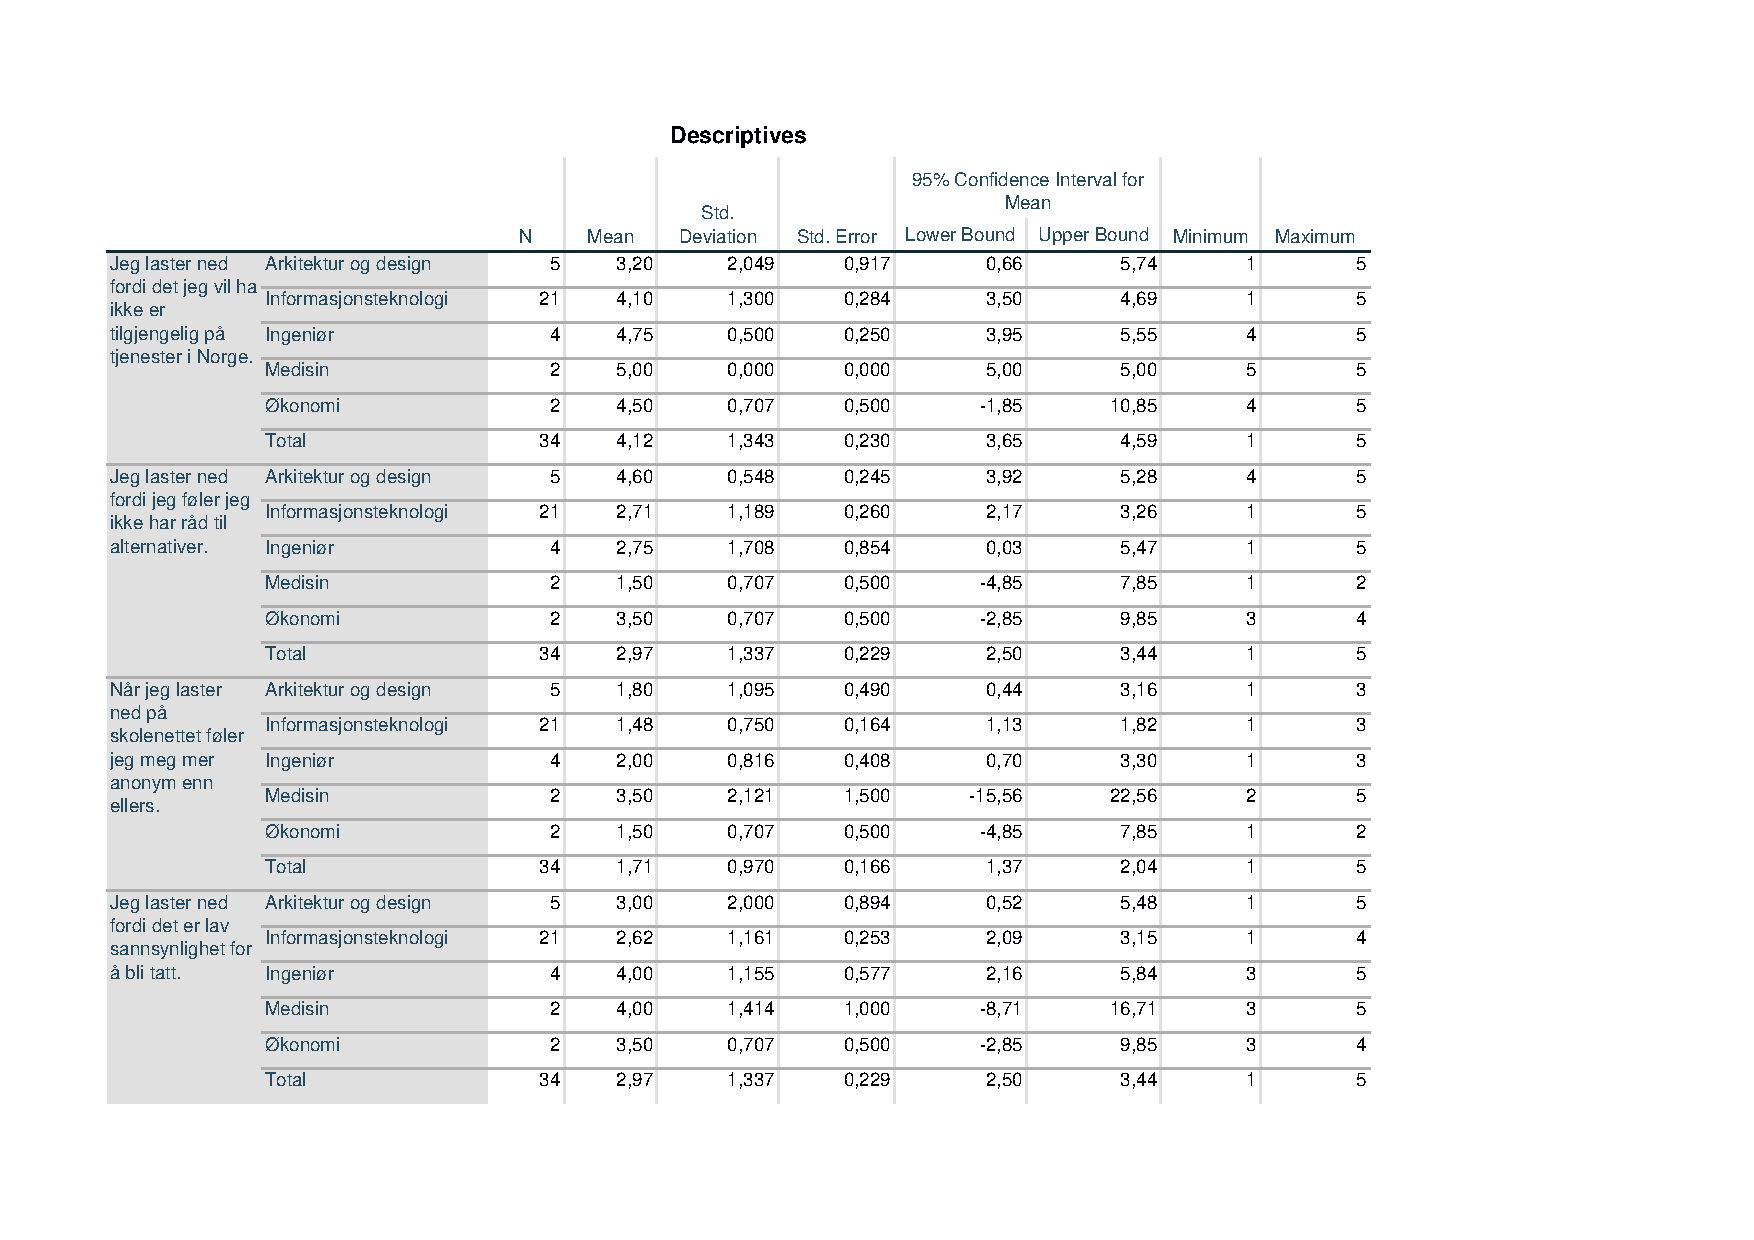
\includegraphics[scale=0.7]{case_1/bilder/DESCRIPTIVES_fakultet-pastand_LIGGENDE.pdf}
    \label{fig:DESCRIPTIVES_fakultet-påstand}
    \caption{Fakultet mot påstander}
\end{figure}


%-----------------------------------------------ANOVA-------------------------------------------------------
\begin{figure}[H]
    \centering
    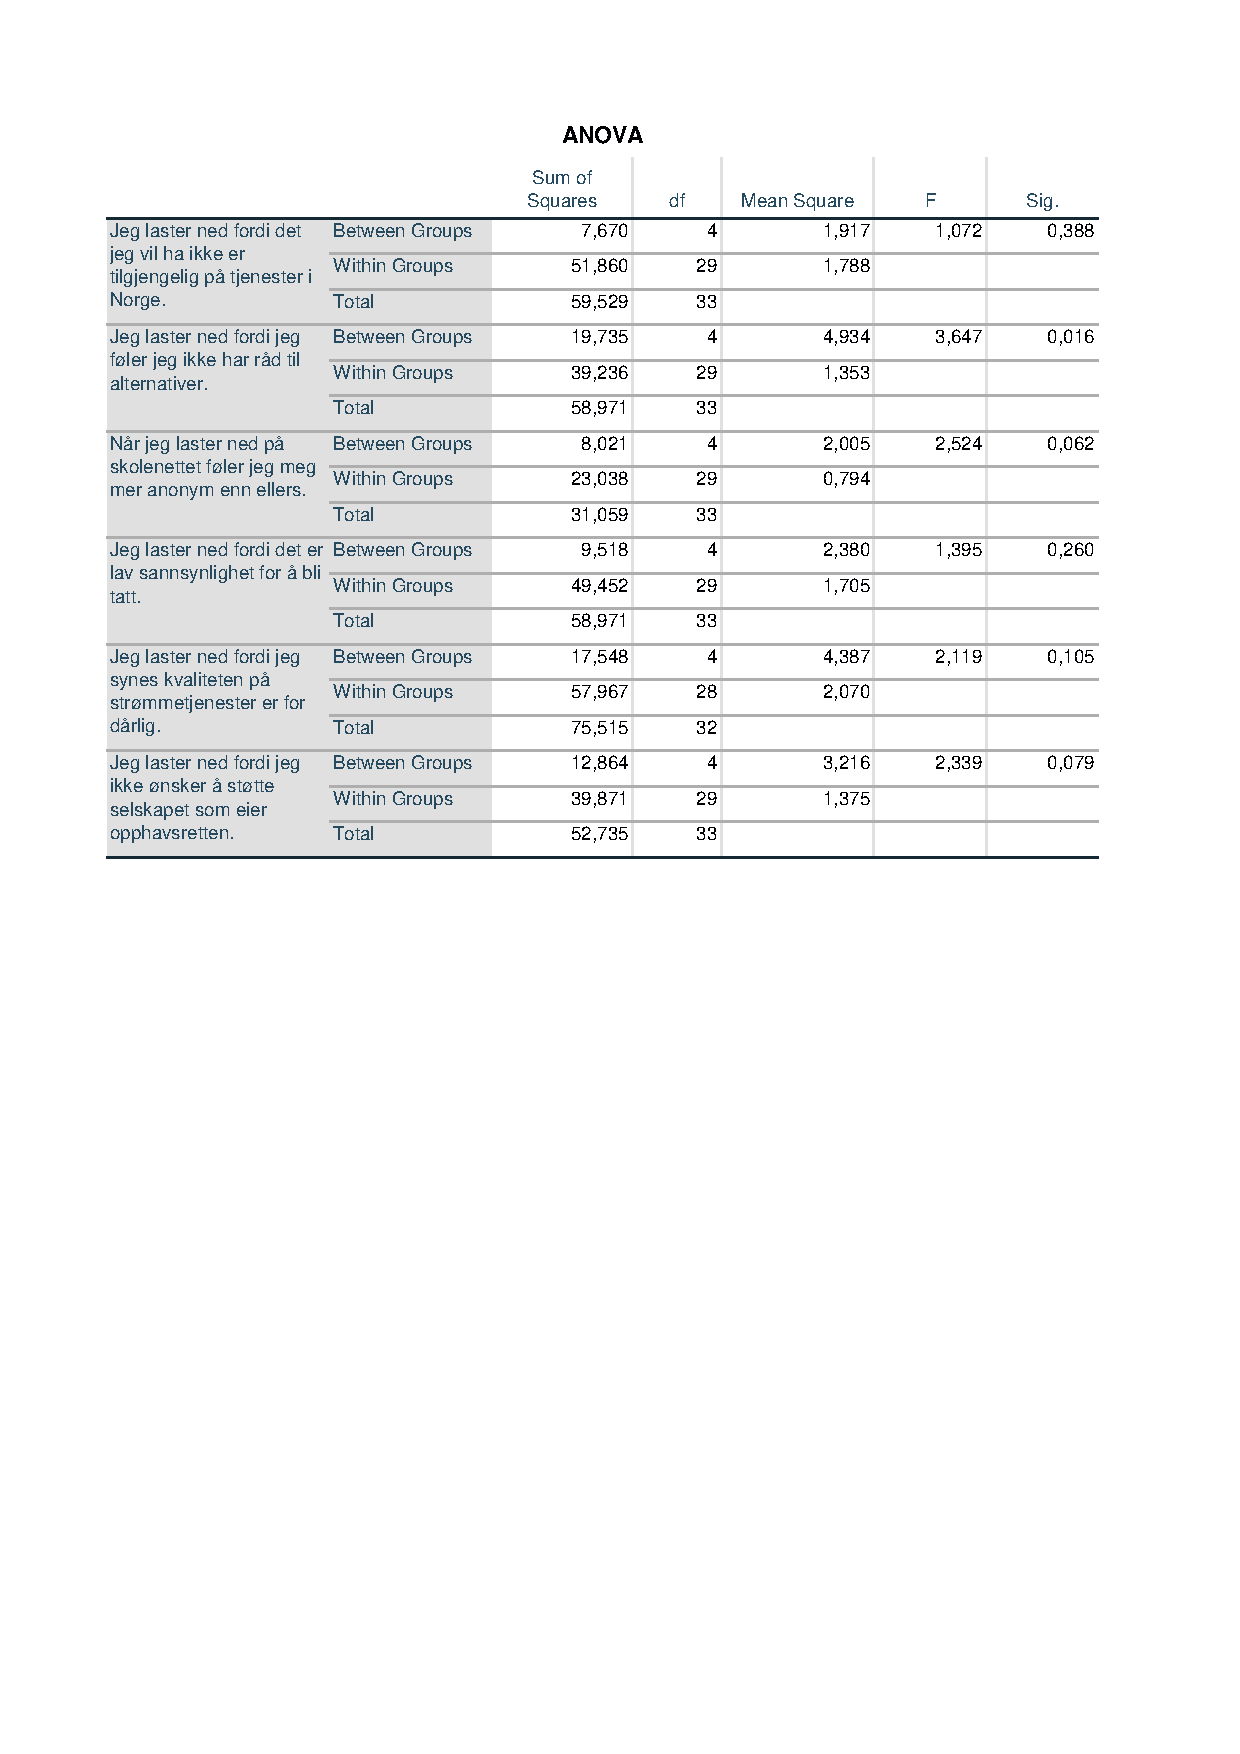
\includegraphics[scale=0.7]{case_1/bilder/ANOVA_fakultet-pastand.pdf}
    \label{fig:ANOVA_fakultet-påstand}
    \caption{Fakultet mot påstander - ANOVA}
\end{figure}


%-----------------------------------------------POST HOC ANALYSE--------------------------------------------
\begin{figure}[H]
    \centering
    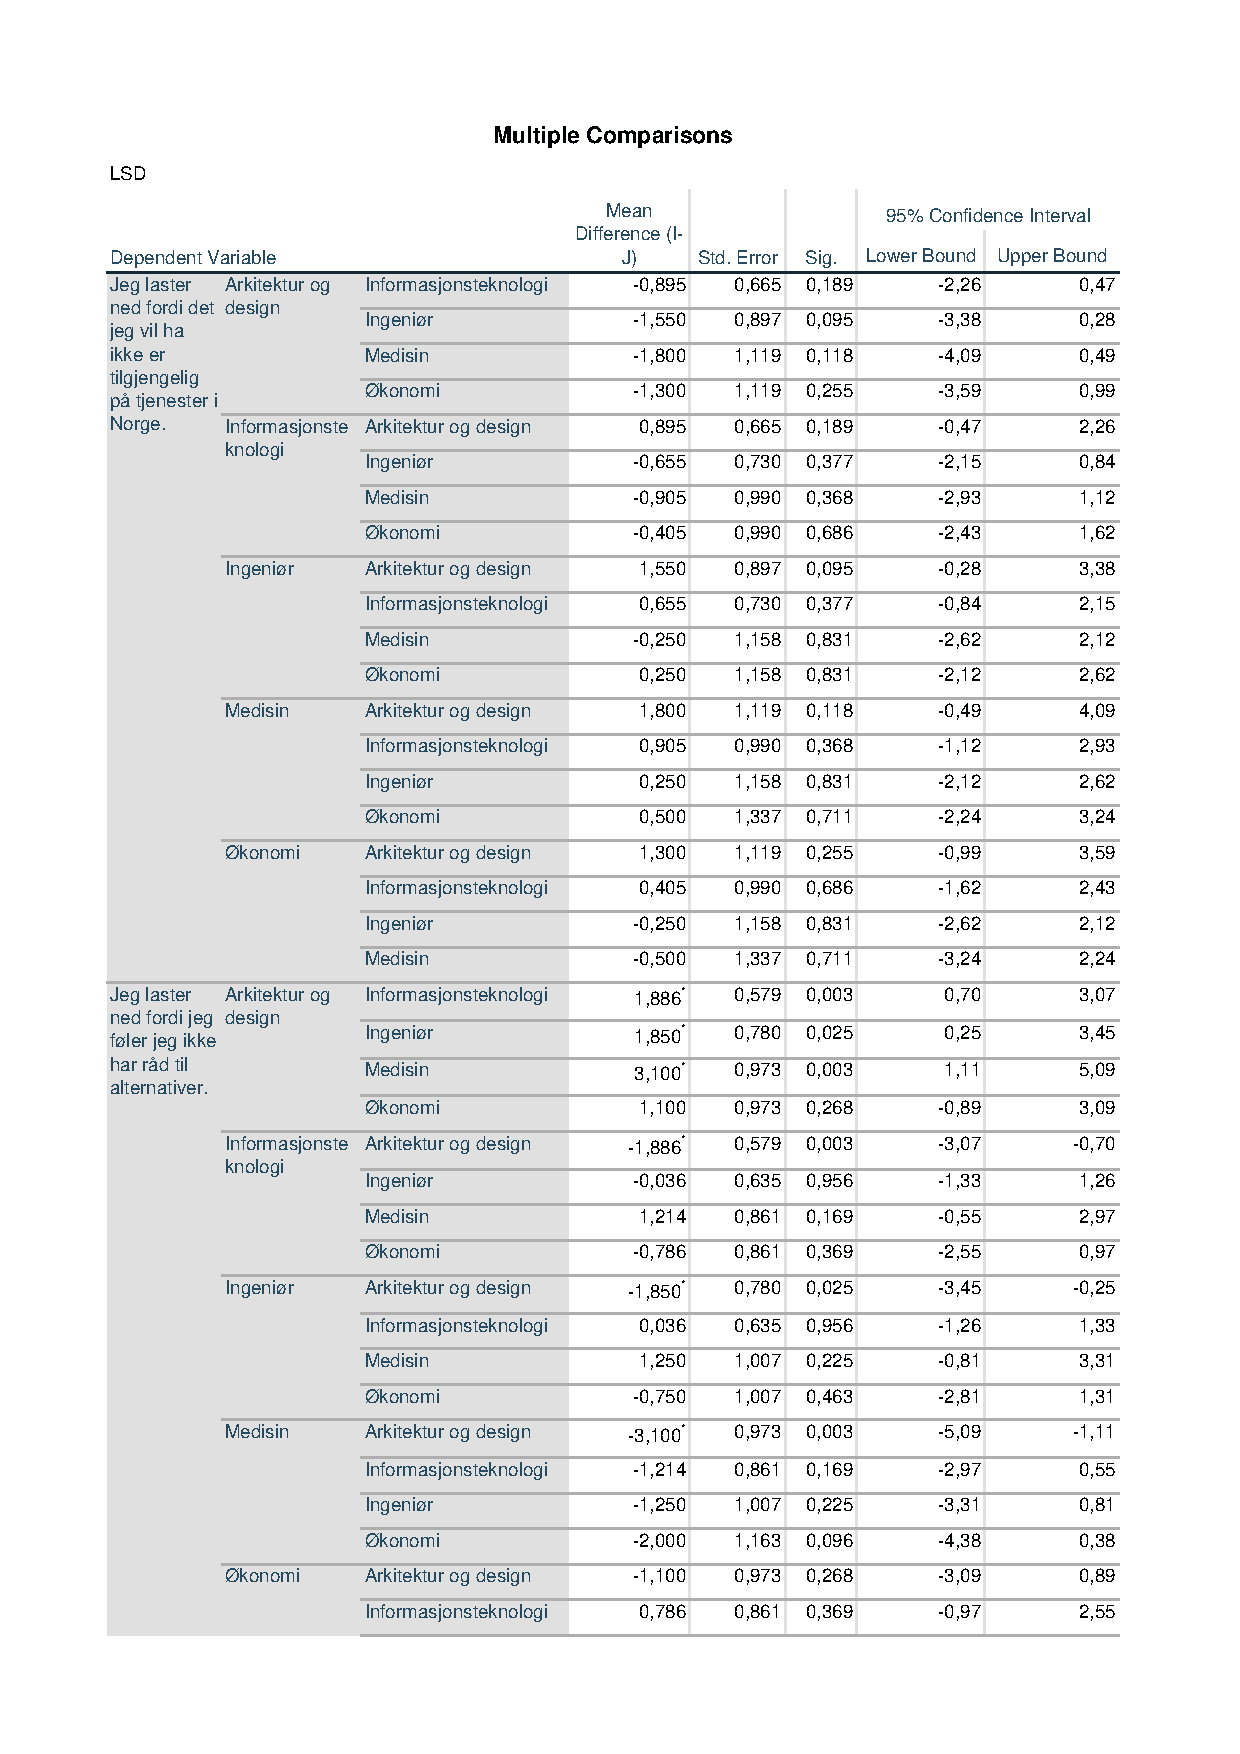
\includegraphics[scale=0.7]{case_1/bilder/Post_Hoc_test_fakultet-pastand.pdf}
    \label{fig:POST-HOC_fakultet-påstand}
    \caption{Fakultet mot påstander - POST HOC}
\end{figure}



%-----------------------------------------------ONEWAY ANOVA - IT/ANDRE MOT PÅSTAND------------------------
%-----------------------------------------------DESCRIPTIVES-----------------------------------------------
\begin{figure}[H]
    \centering
    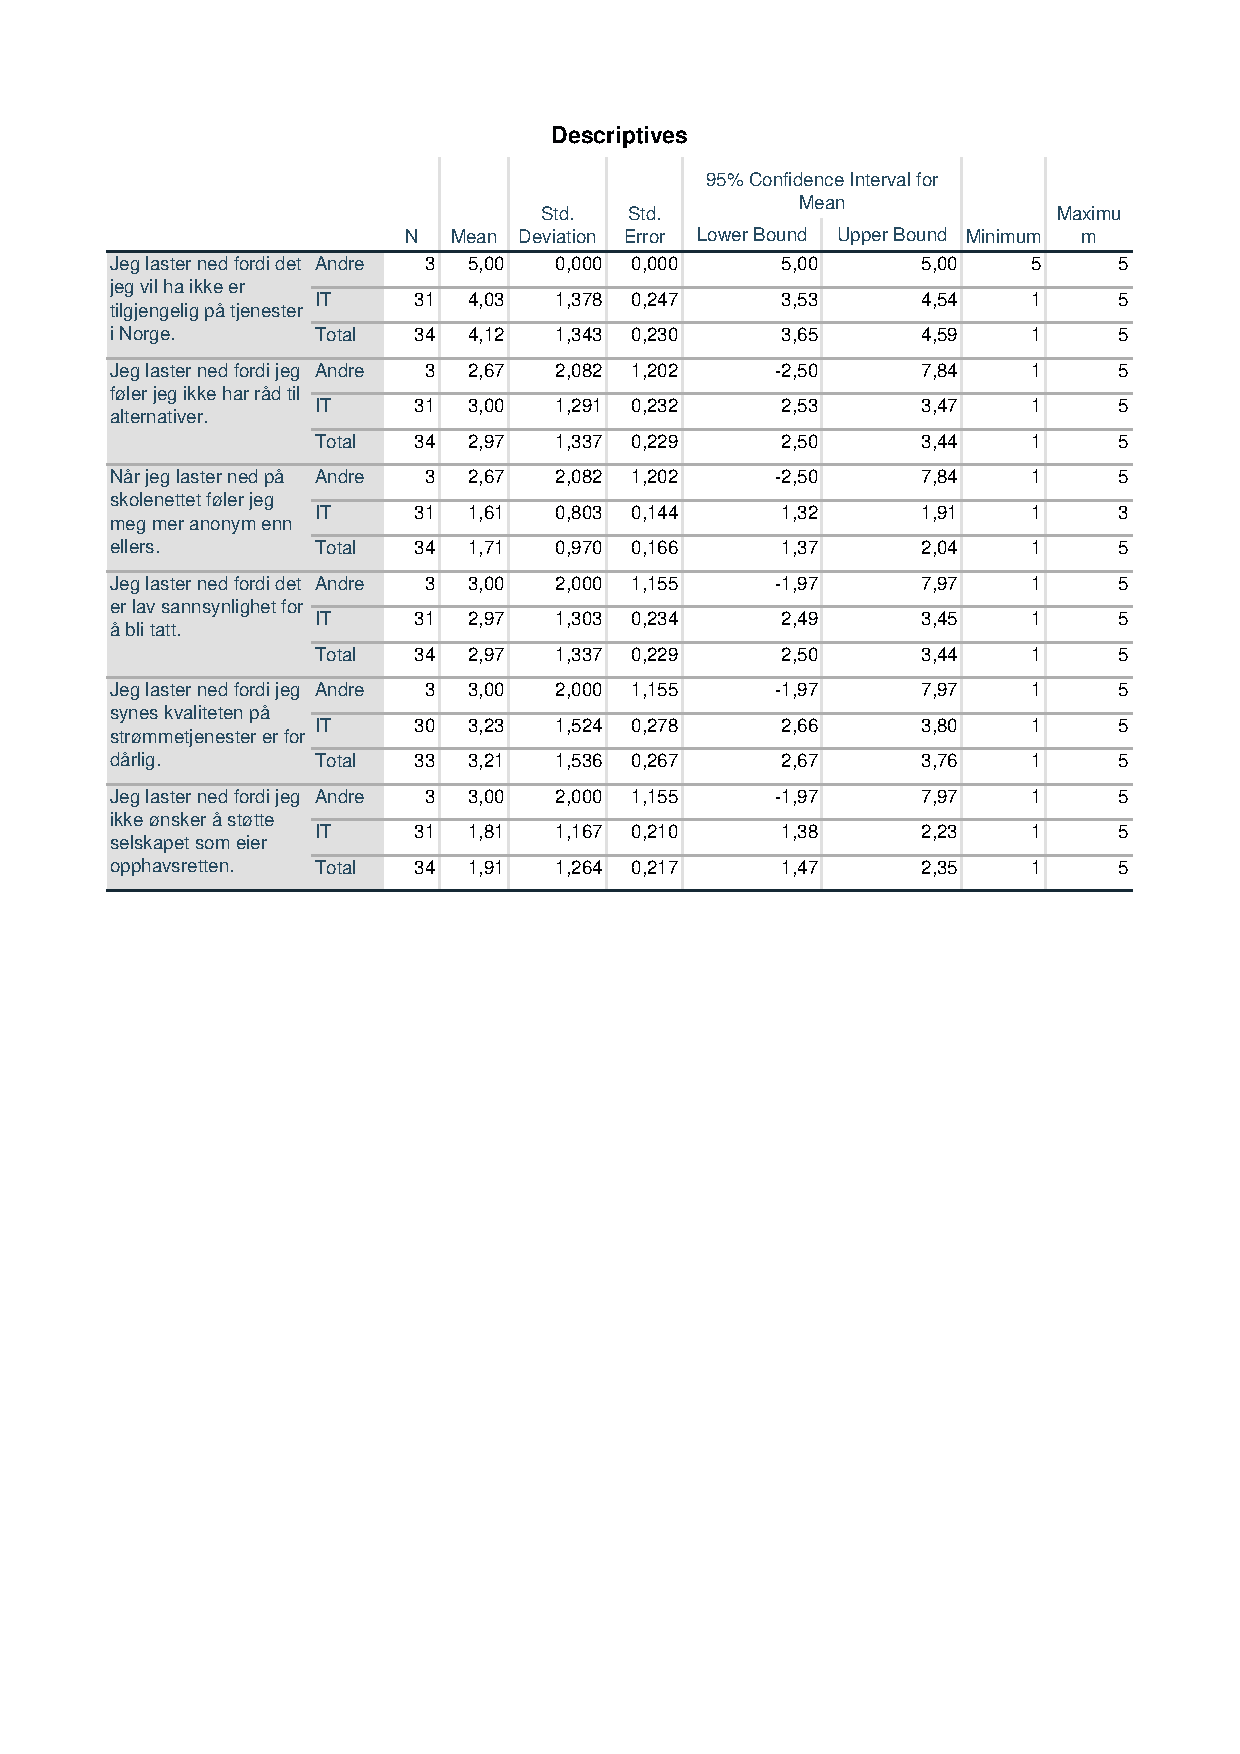
\includegraphics[scale=0.7]{case_1/bilder/DESCRIPTIVES_IT-ANDRE-pastand.pdf}
    \label{fig:DESCRIPTIVES_IT/ANDRE-påstand}
    \caption{Fakultet delt inn i IT og andre mot påstander - DESCRIPTIVES}
    
\end{figure}

%-----------------------------------------------ANOVA-------------------------------------------------------
\begin{figure}[H]
    \centering
    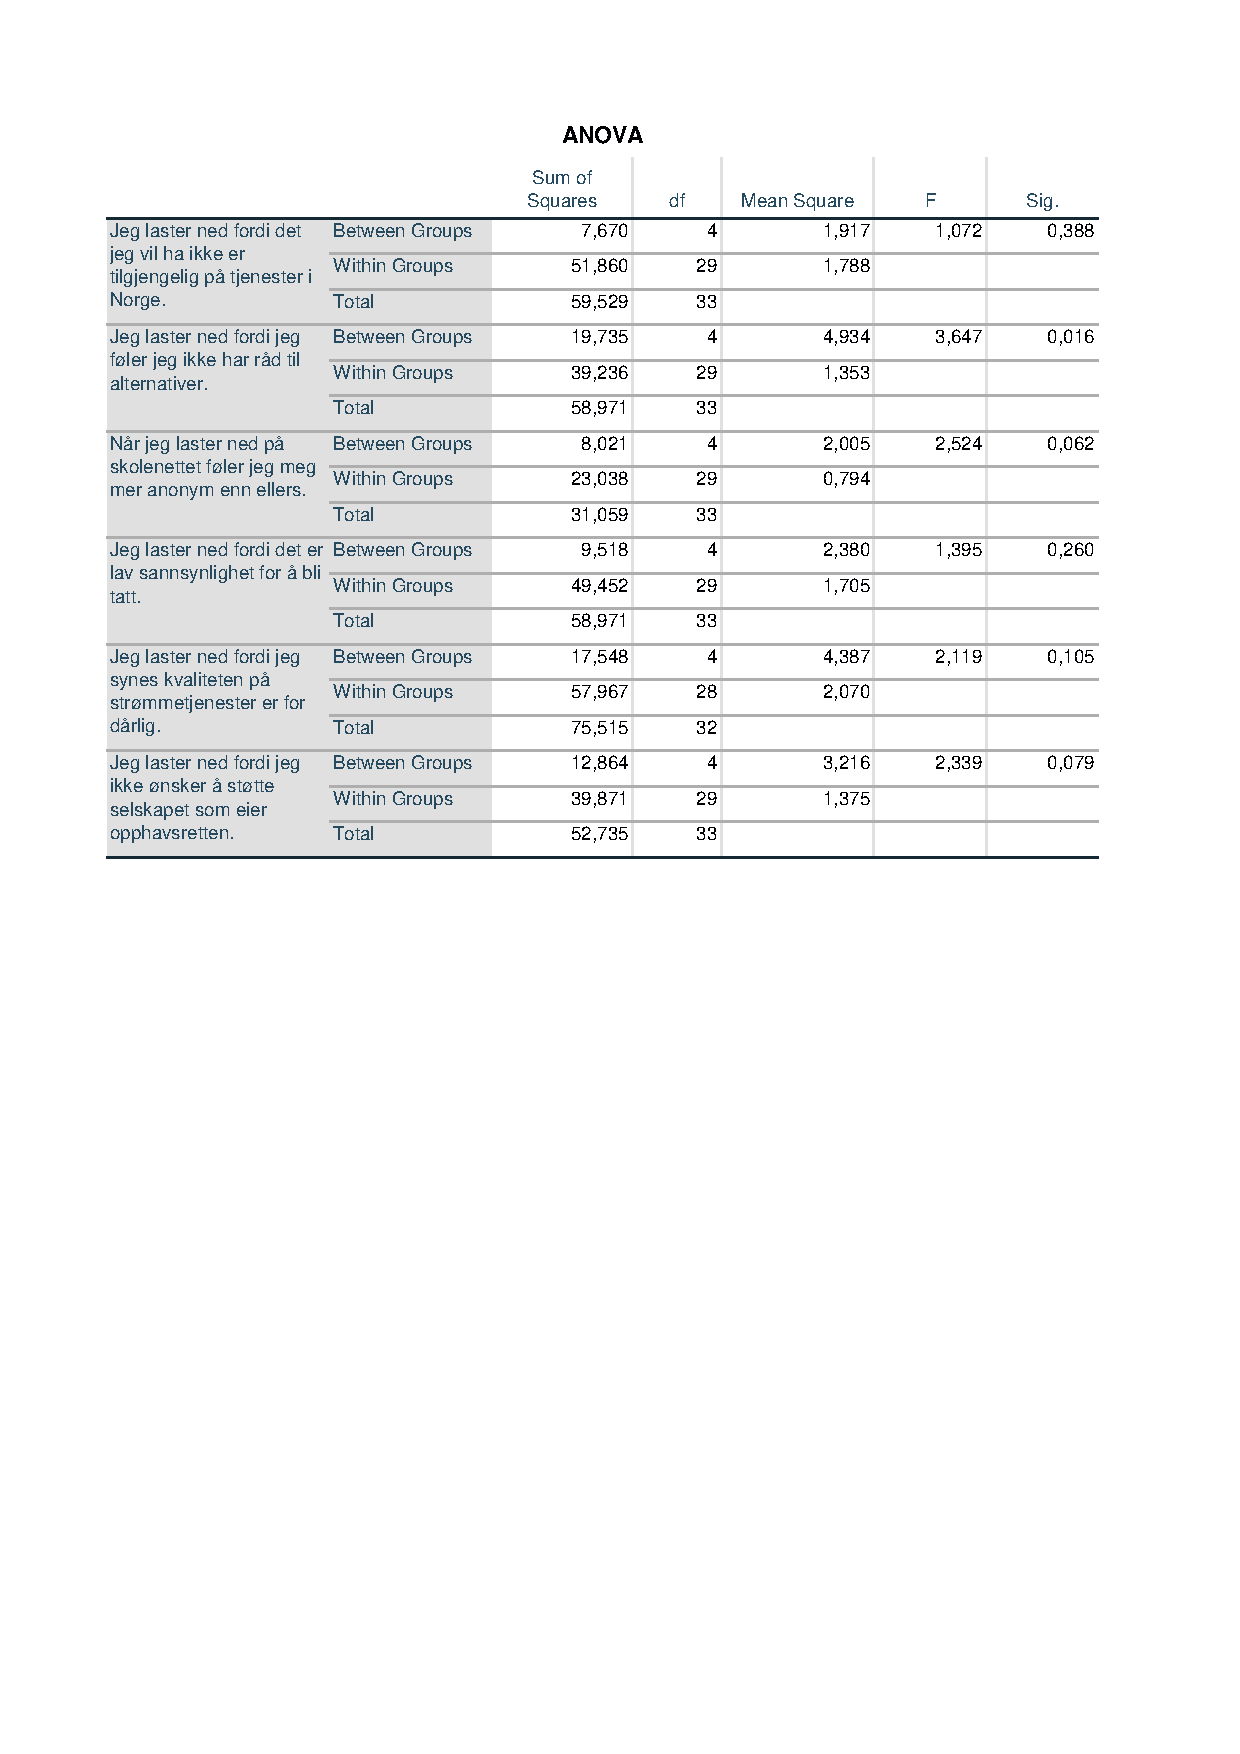
\includegraphics[scale=0.7]{case_1/bilder/ANOVA_fakultet-pastand.pdf}
    \label{fig:ANOVA_IT/ANDRE-påstand}
    \caption{Fakultet delt inn i IT og andre mot påstander - ANOVA}
\end{figure}


